% chapter_2_lit_review.tex
\chapter{Literature Review and Methodological Foundations}
\label{chap:litreview}

\paragraph{Methodology roadmap.} We organize this review by methodology rather than chronology: (i) canonical foundations for margins and spreads (Harville, Stern, state space); (ii) score and margin distributions (Poisson/Skellam, bivariate and dynamic Poisson); (iii) evaluation and calibration (proper scores, reliability); (iv) dependence modeling (copulas) with goodness‑of‑fit and tail checks; and (v) mapping predictive metrics to decision value. Staking theory appears later in Chapter~\ref{chap:risk} to keep Chapter~2 focused on modeling and evaluation.

\section{Canonical Foundations}
We first situate the dissertation with ten canonical works that anchor the modeling, evaluation, and decision layers. For each, we summarize the contribution, give the mathematical core, and note the application to NFL betting markets.

\subsection{Harville (1980): Linear-Model Predictions for NFL} \label{subsec:harville1980}
\sdesc{Proposes linear models for NFL game outcomes, connecting team strengths and covariates to score differential and win probability.}
\mdesc{Let $M_{ij}$ be margin (home $i$ vs away $j$). A two-way design with home advantage $h$ and team effects $\theta_k$ reads}
\begin{equation}\label{eq:harville}
M_{ij} = h + (\theta_i - \theta_j) + \varepsilon,\qquad \varepsilon\sim \mathcal N(0,\sigma^2),
\end{equation}
estimated by (generalized) least squares, with identifiability constraints (e.g., $\sum_k \theta_k=0$). Win probability maps via $\Pr(M_{ij}>0)=\Phi\big((h+\theta_i-\theta_j)/\sigma\big)$.
\appdesc{Equation \eqref{eq:harville} is a baseline for spread pricing and win probability, and underlies state-space generalizations used here.}
\bridge{Margins provide a continuous target; the next step relates posted spreads to win probability so we can compare generative models with market quotes.}

\subsection{Stern (1991): Spread-to-Win Mapping} \label{subsec:stern1991}
\sdesc{Relates posted spreads to win probability under a Gaussian margin model.}
\mdesc{With margin $M\sim\mathcal N(\mu,\sigma^2)$ and spread $p$, we obtain \eqref{eq:stern-win}.}
\appdesc{Empirical $\hat\sigma$ by era links spreads to win odds, and provides a consistency check for classifiers trained on features plus prices.}
\bridge{Knowing how spreads map to win odds, we next ask how team strengths evolve over time, motivating state-space ratings.}

\subsection{Glickman \& Stern (1998): State-Space Team Ratings} \label{subsec:glickman1998}
\sdesc{Time-evolving team strengths with linear-Gaussian state evolution, estimated via Kalman filtering/smoothing.}
\mdesc{For team $k$ strength $\theta_{k,t}$,}
\begin{align}
\theta_{k,t} &= \theta_{k,t-1}+\eta_{k,t}, & \eta_{k,t}&\sim \mathcal N(0,\tau^2),\\
M_t &= h + (\theta_{h(t),t}-\theta_{a(t),t}) + \epsilon_t, & \epsilon_t&\sim \mathcal N(0,\sigma^2),
\end{align}
with standard Kalman recursions for posterior means/variances.  
\appdesc{Supplies temporally stable latent strengths, yielding calibrated priors for spread/win models and robust inputs to score-distribution layers.}
\bridge{Margins summarize outcomes, but pricing totals and correlated bets needs a score model; we therefore introduce Poisson scoring.}

\subsection{Maher (1982): Poisson Goals Model} \label{subsec:maher1982}
\sdesc{Independent Poisson scoring intensities by team/venue; a building block for low-scoring sports.}
\mdesc{$X\sim\mathrm{Pois}(\lambda)$, $Y\sim\mathrm{Pois}(\mu)$ with log-links $\log\lambda = \alpha_i+\beta_j+v_{\text{home}}$, $\log\mu=\alpha'_j+\beta'_i$.}
\appdesc{Although NFL is higher-scoring, the resulting Skellam margin (Section~\ref{subsec:skellam-mom}) remains useful for integer margins, teaser/middle pricing, and key-number analysis.}
\bridge{Independent Poisson can misfit low scores; Dixon--Coles shows how to correct dependence near small counts.}

\subsection{Dixon \& Coles (1997): Dependence and Low-Score Adjustments} \label{subsec:dixon1997}
\sdesc{Poisson framework with adjustments to improve fit in low-score outcomes and time weighting.}
\mdesc{Likelihood reweighting for small-score outcomes modifies a baseline Poisson log-likelihood.}
\appdesc{Motivates reweighting near key margins and era-aware weighting to control leakage and regime drift.}
\bridge{Fixing low-score dependence still assumes independent team scores; next we model positive score correlation via a shared component.}

\subsection{Karlis \& Ntzoufras (2003): Bivariate Poisson} \label{subsec:karlis2003}
\sdesc{Introduces a shared latent component for positively correlated scores.}
\mdesc{$X=U+Z$, $Y=V+Z$ with $U,V,Z\overset{\text{iid}}\sim\mathrm{Pois}(\cdot)$; then $\mathrm{Cov}(X,Y)=\E[Z]=\lambda_0$. The joint pmf admits closed form via trivariate Poisson sums.}
\appdesc{Captures correlated scoring (pace, situational exchanges) and yields coherent joint pricing for correlated parlays.}
\bridge{Correlation and intensities vary through the season; the dynamic bivariate Poisson extends these ideas over time.}

\subsection{Koopman, Lit \& Lucas (2015): Dynamic Bivariate Poisson} \label{subsec:koopman2015}
\sdesc{Evolves attack/defense parameters over time in a state-space framework with non-Gaussian likelihoods.}
\mdesc{Let $\lambda_{i,t}=\exp(x_{i,t}^\top\beta + s_{i,t})$ with latent $s_{i,t}$ following an AR(1); similarly for $\mu_{j,t}$ and a shared $\lambda_{0,t}$. Filtering uses simulation-based methods (e.g., particle filters).}
\appdesc{Adapts joint-score dependence across the season; improves teaser/SGP risk estimates.}
\bridge{For margin-centric pricing and key-number analysis we also need a direct model for integer differences: enter the Skellam distribution.}

\subsection{Skellam (1946): Difference of Two Poissons} \label{subsec:skellam1946}
\sdesc{Closed-form pmf for $D=X-Y$ with $X,Y$ independent Poisson; moments and generating functions.}
\mdesc{See \eqref{eq:skellam-pmf}--\eqref{eq:skellam-moments}; mgf $M_D(t)=\exp\big(\lambda(e^t-1)+\mu(e^{-t}-1)\big)$.}
\appdesc{Natural integer-margin model; a convenient substrate for key-number reweighting and teaser/middle pricing.}
\bridge{Once we can produce calibrated distributions, we must evaluate them properly—hence proper scoring rules.}

\subsection{Gneiting \& Raftery (2007): Proper Scoring Rules} \label{subsec:gneiting2007}
\sdesc{Catalogs proper/strictly proper scoring rules (log-loss, Brier, CRPS) and links calibration to optimality.}
\mdesc{For CDF $F$ and realization $y$, the continuous ranked probability score is}
\begin{equation}
\mathrm{CRPS}(F,y)=\int_{-\infty}^{\infty}\big(F(z)-\mathbb 1\{z\ge y\}\big)^2\,\dd z,
\end{equation}
strictly proper for continuous targets.  
\appdesc{Used for margin/total distributions; we report CRPS and reliability alongside CLV.}
\bridge{Calibrated probabilities and uncertainties ultimately inform actions; we defer staking theory to Chapter~\ref{chap:risk} and proceed to score/margin models next.}

\section{Score and Margin Distributions}
% --- Detailed mathematical exposition: score/margin foundations ---
\subsection{Skellam distribution: construction and moments}\label{subsec:skellam-mom}
The Skellam distribution \citep{skellam1946} arises as the difference of two independent Poisson variates and underpins integer margin modelling. Early football-score models \citep{maher1982,dixon1997} adopt Poisson assumptions to capture low-scoring regimes; extensions to allow dependence \citep{karlis2003,koopman2015} are crucial for joint pricing of spreads and totals.
Let $X\sim\mathrm{Pois}(\lambda)$ and $Y\sim\mathrm{Pois}(\mu)$ independent. The difference
$D=X-Y$ has the Skellam pmf
\begin{equation}\label{eq:skellam-pmf}
\Prob(D=d)=e^{-(\lambda+\mu)}\!\left(\frac{\lambda}{\mu}\right)^{d/2}
\,I_{|d|}\!\big(2\sqrt{\lambda\mu}\big),\qquad d\in\mathbb{Z},
\end{equation}
with $I_\nu(\cdot)$ the modified Bessel function of the first kind. Using pgfs and coefficient
extraction yields \eqref{eq:skellam-pmf}. Its mean/variance are
\begin{equation}\label{eq:skellam-moments}
\E[D]=\lambda-\mu,\qquad \Var(D)=\lambda+\mu.
\end{equation}
It is often convenient to reparametrize by $(\mu_D,\sigma_D^2)=(\lambda-\mu,\lambda+\mu)$ with
$\lambda=\tfrac12(\sigma_D^2+\mu_D)$ and $\mu=\tfrac12(\sigma_D^2-\mu_D)$.

\paragraph{Gaussian limit.} For large $(\lambda,\mu)$ with fixed $(\mu_D,\sigma_D^2)$, the Skellam
distribution approaches $\mathcal{N}(\mu_D,\sigma_D^2)$, motivating probit links between spreads and win probability.

\subsection{Bivariate Poisson: pmf, likelihood, and EM updates}\label{subsec:bp-pmf}
Following \Cref{subsec:karlis2003}, write scores as $X=U+Z$, $Y=V+Z$ with independent
$U\sim\mathrm{Pois}(\lambda_1)$, $V\sim\mathrm{Pois}(\lambda_2)$, $Z\sim\mathrm{Pois}(\lambda_0)$. Then
\begin{align}
\Pr(X=x,Y=y)
&= e^{-(\lambda_0+\lambda_1+\lambda_2)}\sum_{z=0}^{\min(x,y)} \notag\\[-2pt]
&\quad \tfrac{\lambda_0^z}{z!}\,\tfrac{\lambda_1^{x-z}}{(x-z)!}\,\tfrac{\lambda_2^{y-z}}{(y-z)!},\label{eq:bp-pmf}\\[-2pt]
\Cov(X,Y) &= \lambda_0,\quad \E[X]=\lambda_0+\lambda_1,\quad \E[Y]=\lambda_0+\lambda_2.
\end{align}
For observations $\{(x_i,y_i)\}$ the log-likelihood is $\ell(\boldsymbol\lambda)=\sum_i \log \Pr(X=x_i,Y=y_i)$ with \eqref{eq:bp-pmf}. A convenient EM arises by treating $Z_i\sim\mathrm{Pois}(\lambda_0)$ as latent:
\begin{align}
\text{E-step: } &\ w_{i,z}=\Pr(Z_i=z\mid x_i,y_i;\boldsymbol\lambda) \propto \notag\\[-2pt]
&\quad \tfrac{\lambda_0^z}{z!}\,\tfrac{\lambda_1^{x_i-z}}{(x_i-z)!}\,\tfrac{\lambda_2^{y_i-z}}{(y_i-z)!},\label{eq:bp-weights}\\
\text{M-step: } &\ \lambda_0^{\text{new}}=\frac{1}{n}\sum_i \sum_{z=0}^{m_i} z\,w_{i,z},\notag\\[-2pt]
&\ \lambda_1^{\text{new}}=\frac{1}{n}\sum_i \sum_{z=0}^{m_i} (x_i-z)\,w_{i,z},\notag\\[-2pt]
&\ \lambda_2^{\text{new}}=\frac{1}{n}\sum_i \sum_{z=0}^{m_i} (y_i-z)\,w_{i,z},
\end{align}
where $m_i=\min(x_i,y_i)$. In practice we maximize the conditional expectation of the complete-data log-likelihood.

\paragraph{Toy numeric.} For $(x,y)=(2,1)$ and $(\lambda_0,\lambda_1,\lambda_2)=(0.3,1.4,1.1)$,
\[\Pr(X=2,Y=1)=e^{-2.8}\Big(\tfrac{\lambda_0^0\lambda_1^2\lambda_2^1}{2!1!}+\tfrac{\lambda_0^1\lambda_1^1\lambda_2^0}{1!1!0!}\Big)\approx e^{-2.8}\,(1.078+0.42)\approx 0.216,\]
illustrating the latent $Z$ mixing across $z=0,1$.

\section{From Spreads and Totals to Probabilities}
\subsection{Stern’s spread-to-win map: full derivation}\label{subsec:stern-derivation}
We connect posted spreads to win probabilities following \citet{stern1991}, which motivates probit links in baseline classifiers.
Assume the realized margin $M$ satisfies $M=\mu+\varepsilon$ with $\varepsilon\sim\mathcal{N}(0,\sigma^2)$. If the posted spread is $p$
(favorite $-p$), then
\begin{equation}\label{eq:stern-win}
\Prob(\text{favorite wins})=\Prob(M>0)=\Phi\!\Big(\frac{\mu}{\sigma}\Big),\qquad
\Prob(\text{favorite covers})=\Phi\!\Big(\frac{\mu-p}{\sigma}\Big).
\end{equation}
\begingroup\sloppy
Under efficiency for the mean $\mu\approx p$ we get the classical approximation
$\Prob(\text{win})\approx\Phi(p/\sigma)$. Empirically we estimate $\sigma$ with a probit regression of win indicators on posted spreads; we report $\hat\sigma$ by season/era.
\endgroup

\begin{example}[Worked mapping]
If the market posts $p=3$ and historical fit yields $\hat\sigma=13.5$, then Stern’s map gives
$\Pr(\text{win})\approx\Phi(3/13.5)\approx 0.59$. The implied moneyline fair odds are roughly $1/0.59\approx1.69$ (decimal), before vig and correlation adjustments.
\end{example}

\subsection{Dixon--Coles low-score adjustment vs key-number reweighting}\label{subsec:dc-vs-keys}
\begin{sloppypar}
\Cref{subsec:dixon1997} introduces a small-score weighting to correct dependence/misspecification in low-goal outcomes.
Let $L(\lambda,\mu)$ denote the Poisson log-likelihood and $w(x,y;\kappa)$ a down/up-weighting for $(x,y)\in\{0,1\}^2$ (tuning $\kappa$).
The adjusted log-likelihood reads
\[\ell_{\text{DC}}(\lambda,\mu,\kappa)=\sum_i w(x_i,y_i;\kappa)\,\log \Pr(X=x_i,Y=y_i\mid \lambda,\mu)+\text{const},\]
\end{sloppypar}
improving fit for small counts.
In contrast, NFL margins concentrate on \emph{key integers} (3, 6, 7, 10). Rather than reweight small \emph{scores}, we reweight the \emph{margin pmf} $q(d)$ multiplicatively to match empirical key masses while preserving location/scale via \eqref{eq:reweight-ls}. This directly addresses teaser/middle pricing where integer masses drive EV.

\subsection{Key-number reweighting as constrained projection}\label{subsec:key-reweight}
Let $q(d)$ be a baseline integer pmf (Skellam or discretized Gaussian) for the margin $D$ and let
$\mathcal{K}=\{3,6,7,10\}$. We seek nonnegative weights $\{w_d\}$ s.t. $\tilde q(d)=w_d q(d)$ is a
pmf matching empirical key masses $\{m_k\}_{k\in\mathcal{K}}$:
\begin{align}\label{eq:reweight-ls}
\min_{\{w_d\ge0\}} \quad & \sum_{k\in\mathcal{K}} \big(w_k q(k)-m_k\big)^2 \\
\text{s.t.}\quad &
\sum_{d} w_d q(d)=1,\quad
\sum_d d\,w_d q(d)=\mu_D,\quad
\sum_d (d-\mu_D)^2 w_d q(d)=\sigma_D^2. \nonumber
\end{align}
The last two constraints preserve mean/variance so reweighting changes shape, not location/scale.
In matrix form, \eqref{eq:reweight-ls} is a small convex QP; if only normalization and key masses
are imposed it has a closed form via Lagrange multipliers. We use $\tilde q$ for teaser/middle pricing in Chapter~\ref{chap:sim}.

\paragraph{Convergence and complexity.} For the projected‑update routine (\Cref{alg:key-reweight}), the objective $\sum_{k\in\mathcal K}(w_k q(k)-m_k)^2$ is convex in $w$, and the projection onto linear moment constraints is nonexpansive; with a fixed step size $\eta\in(0,2/L)$ where $L=\max_k 2 q(k)^2$, the sequence of objective values decreases monotonically and converges to the minimum over the feasible set. Each iteration costs $O(|\mathcal K|+|\mathrm{supp}(q)|)$ to update gradients and solve the $3\times3$ projection system; with a banded support (e.g., $d\in[-40,40]$) this is $O(1)$ per iteration in practice.

For the KL‑tilting alternative (\Cref{subsec:key-kl}), the dual is smooth and strictly concave; Newton or projected gradient (with backtracking) converges to the unique optimum because the log‑partition function is strictly convex. Each dual gradient/Hessian evaluation requires a pass over the support to compute normalizers and moments.

\paragraph{Reference code (Python‑like).}
\begin{verbatim}
def reweight_q(q, keys, targets, mu, var, iters=200, eta=1e-3):
    # q: dict margin->prob; keys: list of ints; targets: dict key->mass
    w = {d: 1.0 for d in q}
    for _ in range(iters):
        # gradient on keys only
        g = {d: 0.0 for d in q}
        for k in keys:
            g[k] = 2.0 * (w[k]*q[k] - targets[k]) * q[k]
        # gradient step + nonnegativity
        for d in q:
            w[d] = max(0.0, w[d] - eta*g[d])
        # project to normalization + moments via affine update w <- w + a + b d + c (d-mu)^2
        A = [[sum(q[d] for d in q),        sum(d*q[d] for d in q),        sum((d-mu)**2*q[d] for d in q)],
             [sum(q[d] for d in q),        sum(d*q[d] for d in q),        sum((d-mu)**2*q[d] for d in q)],
             [sum(q[d] for d in q),        sum(d*q[d] for d in q),        sum((d-mu)**2*q[d] for d in q)]]
        # In practice compute A and rhs properly; solve for (a,b,c) and update w
        # ... (omitted: 3x3 linear solve)
    return {d: w[d]*q[d] for d in q}
\end{verbatim}

\paragraph{Feasibility and stability.}\label{subsec:key-feas}
Write $v(d)=(1,\,d,\,(d-\mu_D)^2,\,\mathbb{1}\{d=k: k\in\mathcal{K}\})^\top$ and $\bar v=\sum_d q(d) v(d)$ for baseline moments and key masses. The feasible set is the convex cone of achievable moments $\mathcal{V}=\{\sum_d w_d q(d) v(d): w_d\ge0\}$. If the target vector $v^\star=(1,\,\mu_D,\,\sigma_D^2,\,\{m_k\})$ lies outside $\mathcal{V}$ (e.g., key masses too large relative to support), we solve a penalized problem with nonnegative slacks:
\begin{align*}
\min_{\{w_d\ge0\},\,s\ge0}\quad & \sum_{k\in\mathcal{K}} \big(w_k q(k)-m_k\big)^2 + \lambda\,\|s\|_2^2\\
\text{s.t.}\quad & \sum_d w_d q(d)=1,\ \sum_d d\,w_d q(d)=\mu_D,\ \sum_d (d-\mu_D)^2 w_d q(d)=\sigma_D^2+s,
\end{align*}
and declare infeasibility if $\|s\|$ exceeds a tolerance. This guards against unstable weights when targets are unrealistic.

\paragraph{KL‑tilting alternative (maximum entropy).}\label{subsec:key-kl}
An alternative with strong existence/positivity guarantees is multiplicative tilting that minimizes KL divergence to $q$:
\begin{align*}
\min_{\tilde q}\quad & \sum_d \tilde q(d)\log\frac{\tilde q(d)}{q(d)}\\
\text{s.t.}\quad & \sum_d \tilde q(d)=1,\ \sum_d d\,\tilde q(d)=\mu_D,\ \sum_d (d-\mu_D)^2\tilde q(d)=\sigma_D^2,\ \tilde q(k)=m_k\ (k\in\mathcal{K}).
\end{align*}
By convex duality, the solution has exponential form
\[
\tilde q_\alpha(d)\propto q(d)\exp\{\alpha_0+\alpha_1 d+\alpha_2 (d-\mu_D)^2+\sum_{k\in\mathcal{K}}\delta_k\,\mathbb{1}\{d=k\}\},
\]
with multipliers $\alpha,\delta$ found by Newton or projected gradient on the dual. This preserves support and strict positivity and converges under standard step‑size conditions. In practice we attempt KL‑tilting first and fall back to the QP with slacks if key targets violate convex‑hull constraints.

\begin{algorithm}[t]
  \caption{Key-number reweighting via projected updates}
  \label{alg:key-reweight}
  \begin{algorithmic}[1]
    \Require baseline pmf $q(d)$ on $\mathbb{Z}$; key set $\mathcal{K}$ with targets $m_k$; target moments $(\mu_D,\sigma_D^2)$; step size $\eta$
    \State initialize $w_d\leftarrow 1$ for all $d$; repeat for $T$ iters
    \State gradient on keys: for $k\in\mathcal{K}$, \; $g_k \leftarrow 2\big(w_k q(k)-m_k\big)\,q(k)$; set $g_d\leftarrow 0$ otherwise
    \State gradient step: $w_d \leftarrow \max\{0,\; w_d - \eta g_d\}$
    \State project to constraints: solve for multipliers $(\alpha,\beta,\gamma)$ s.t.
      $\sum_d w_d q(d)=1$, $\sum_d d\,w_d q(d)=\mu_D$, $\sum_d (d-\mu_D)^2 w_d q(d)=\sigma_D^2$;
      update $w_d \leftarrow \max\{0,\; w_d + \alpha + \beta d + \gamma (d-\mu_D)^2\}$
    \State \textbf{until} convergence of $\sum_{k\in\mathcal{K}}|w_k q(k)-m_k|$
    \State \Return reweighted pmf $\tilde q(d)=w_d q(d)$
  \end{algorithmic}
\end{algorithm}

\section{Paired-Comparison and Dynamic Rating Models}
\label{sec:paired}
Paired-comparison models such as Bradley--Terry \citep{bradleyterry1952} and time-evolving ratings (Elo \citep{elo1978}, state-space \citep{glickman1998}) provide interpretable strength estimates. For American football, linear-Gaussian state evolution \citep{glickman1998} balances responsiveness with stability; ridge penalties or Bayesian priors control variance.

\subsection{Kalman filter equations and worked example}\label{subsec:kalman-derivation}
Under the linear-Gaussian model of \Cref{subsec:glickman1998}, let $m_{t|t-1}$ and $P_{t|t-1}$ be prior mean/variance for the home-away difference; observation variance is $\sigma^2$. The Kalman gain and posterior updates are
\begin{align}
K_t&=\frac{P_{t|t-1}}{P_{t|t-1}+\sigma^2},\qquad m_{t|t}=m_{t|t-1}+K_t\,(M_t-m_{t|t-1}),\\
P_{t|t}&=(1-K_t)P_{t|t-1},\qquad m_{t+1|t}=m_{t|t},\quad P_{t+1|t}=P_{t|t}+\tau^2.
\end{align}
\textit{Example.} With $m_{t|t-1}=1.5$, $P_{t|t-1}=9$, $\sigma^2=36$, observed margin $M_t=6$, we have $K_t=0.2$, $m_{t|t}=1.5+0.2\cdot 4.5=2.4$, $P_{t|t}=7.2$. This posterior feeds spread/win mapping via \Cref{subsec:stern1991}.

\section{Dependence Between Margin and Total}
\subsection{Spread–Total Dependence via Copulas}\label{subsec:copula-st}
We model dependence between margin $M$ and total $T$ to price correlated legs coherently. A convenient baseline is the \emph{Gaussian copula} \citep{nelsen2006}:
$(Z_1,Z_2)\sim \mathcal{N}(\mathbf 0,\begin{psmallmatrix}1&\rho\\ \rho&1\end{psmallmatrix})$, set $(U,V)=(\Phi(Z_1),\Phi(Z_2))$, then $(M,T)=\big(F_M^{-1}(U),F_T^{-1}(V)\big)$. The joint exceedance for teaser legs $A=\{M>p_1\}$, $B=\{T>q_1\}$ is
\[
\Prob(A\cap B)=\iint 1\!\{F_M^{-1}(u)>p_1,\ F_T^{-1}(v)>q_1\}\,c_\rho(u,v)\,\dd u\,\dd v,
\]
with density $c_\rho$. For Gaussian copulas, Kendall’s $\tau$ and $\rho$ relate by $\tau=\tfrac{2}{\pi}\arcsin(\rho)$, which we use to estimate $\rho$ robustly from rank correlation.

\paragraph{Tail behavior and $t$-copulas.} Gaussian copulas have \emph{zero tail dependence}, potentially understating joint tail risk for extreme margins/totals. A heavier-tailed alternative is the \emph{$t$-copula} with correlation $\rho$ and degrees of freedom $\nu$, whose upper/lower tail dependence is
\[
\lambda_U=\lambda_L=2\,t_{\nu+1}\!\left(-\sqrt{\frac{(\nu+1)(1-\rho)}{1+\rho}}\,\right),
\]
where $t_{\nu+1}$ is the $t$ CDF. We use Gaussian copulas for calibration and $t$-copulas in stress tests to bound teaser/SGP risk under stronger tail co-movement.\footnote{See \citet{joe1997} for dependence measures and tail behavior; $t$-copulas are widely used for stress scenarios (e.g., Demarta--McNeil, 2005).}

\paragraph{Estimation.} We estimate $\tau$ (or Spearman’s $\rho_S$) on historical $(M,T)$, map to $\rho$, and evaluate $\Prob(A\cap B)$ by quasi-Monte Carlo. Marginal CDFs $F_M,F_T$ are taken from the fitted Skellam/bivariate-Poisson layers (with key-number reweighting; \Cref{subsec:key-reweight}).

\paragraph{Goodness-of-fit and tail diagnostics.}\label{subsec:copula-gof}
Let $\{(M_t,T_t)\}_{t=1}^n$ be margins/totals and $\hat F_M,\hat F_T$ the fitted marginals. Define pseudo-observations $U_t=\hat F_M(M_t)$, $V_t=\hat F_T(T_t)$. Write $\hat C_n(u,v)=\tfrac1n\sum_{t=1}^n \mathbb{1}\{U_t\le u,\,V_t\le v\}$ for the empirical copula and $C_\theta$ the parametric copula (Gaussian or $t$ with parameter $\theta$).
We assess fit with the Cramér–von Mises functional
\[
S_n= n\int_{[0,1]^2}\big(\hat C_n(u,v)-C_{\hat\theta}(u,v)\big)^2\,\mathrm d C_{\hat\theta}(u,v),
\]
approximated on a grid or via Monte Carlo under $C_{\hat\theta}$. As a complementary check, apply the Rosenblatt transform $W_t=\big(U_t,\, C_{\hat\theta}(V_t\mid U_t)\big)$ and test for i.i.d.\ uniforms (e.g., univariate CvM on each coordinate and independence via a rank test). Consistent rejections motivate switching between Gaussian and $t$ families.

Tail behavior is summarized by the upper/lower tail coefficients
\[
\lambda_U=\lim_{u\uparrow 1}\Pr\big(V>u\mid U>u\big),\qquad
\lambda_L=\lim_{u\downarrow 0}\Pr\big(V\le u\mid U\le u\big),
\]
estimated empirically by high/low quantile counts. Gaussian copulas imply $\lambda_U=\lambda_L=0$; $t$‑copulas yield $\lambda_U=\lambda_L>0$ depending on $\nu$ and $\rho$. We report $(\hat\lambda_U,\hat\lambda_L)$ with block bootstrap intervals to decide whether heavy‑tailed dependence is required.

\begin{algorithm}[t]
  \caption{Copula GOF and Tail Diagnostics}
  \label{alg:copula-gof}
  \begin{algorithmic}[1]
    \Require paired margins/totals $\{(M_t,T_t)\}_{t=1}^n$; fitted marginals $\hat F_M,\hat F_T$; copula family $C_\theta$
    \Ensure CvM statistic $S_n$; Rosenblatt uniformity p‑values; tail coefficients $(\hat\lambda_U,\hat\lambda_L)$ with CIs
    \State Compute pseudo‑obs $U_t\leftarrow\hat F_M(M_t)$, $V_t\leftarrow\hat F_T(T_t)$
    \State Fit $\hat\theta\leftarrow\arg\max_\theta\sum_t \log c_\theta(U_t,V_t)$ (inversion of $\tau$ for Gaussian/$t$)
    \State Empirical copula $\hat C_n(u,v)\leftarrow n^{-1}\sum_t\mathbb{1}\{U_t\le u,V_t\le v\}$
    \State CvM statistic $S_n\leftarrow n\int(\hat C_n-C_{\hat\theta})^2\,\mathrm d C_{\hat\theta}$ (grid or MC)
    \State Rosenblatt transform $W_t\leftarrow(U_t,\, C_{\hat\theta}(V_t\mid U_t))$; test each coord for $\mathrm{Unif}(0,1)$ and independence
    \State Estimate tails: $\hat\lambda_U\leftarrow\frac{\#\{U_t>u_0, V_t>u_0\}}{\#\{U_t>u_0\}}$ as $u_0\uparrow1$; similarly for $\hat\lambda_L$ with $u_0\downarrow0$
    \State Block bootstrap seasonal blocks to get CIs for $(S_n,\hat\lambda_U,\hat\lambda_L)$
  \end{algorithmic}
\end{algorithm}

% Gaussian-copula joint exceedance vs correlation
\begin{figure}[t]
  \centering
  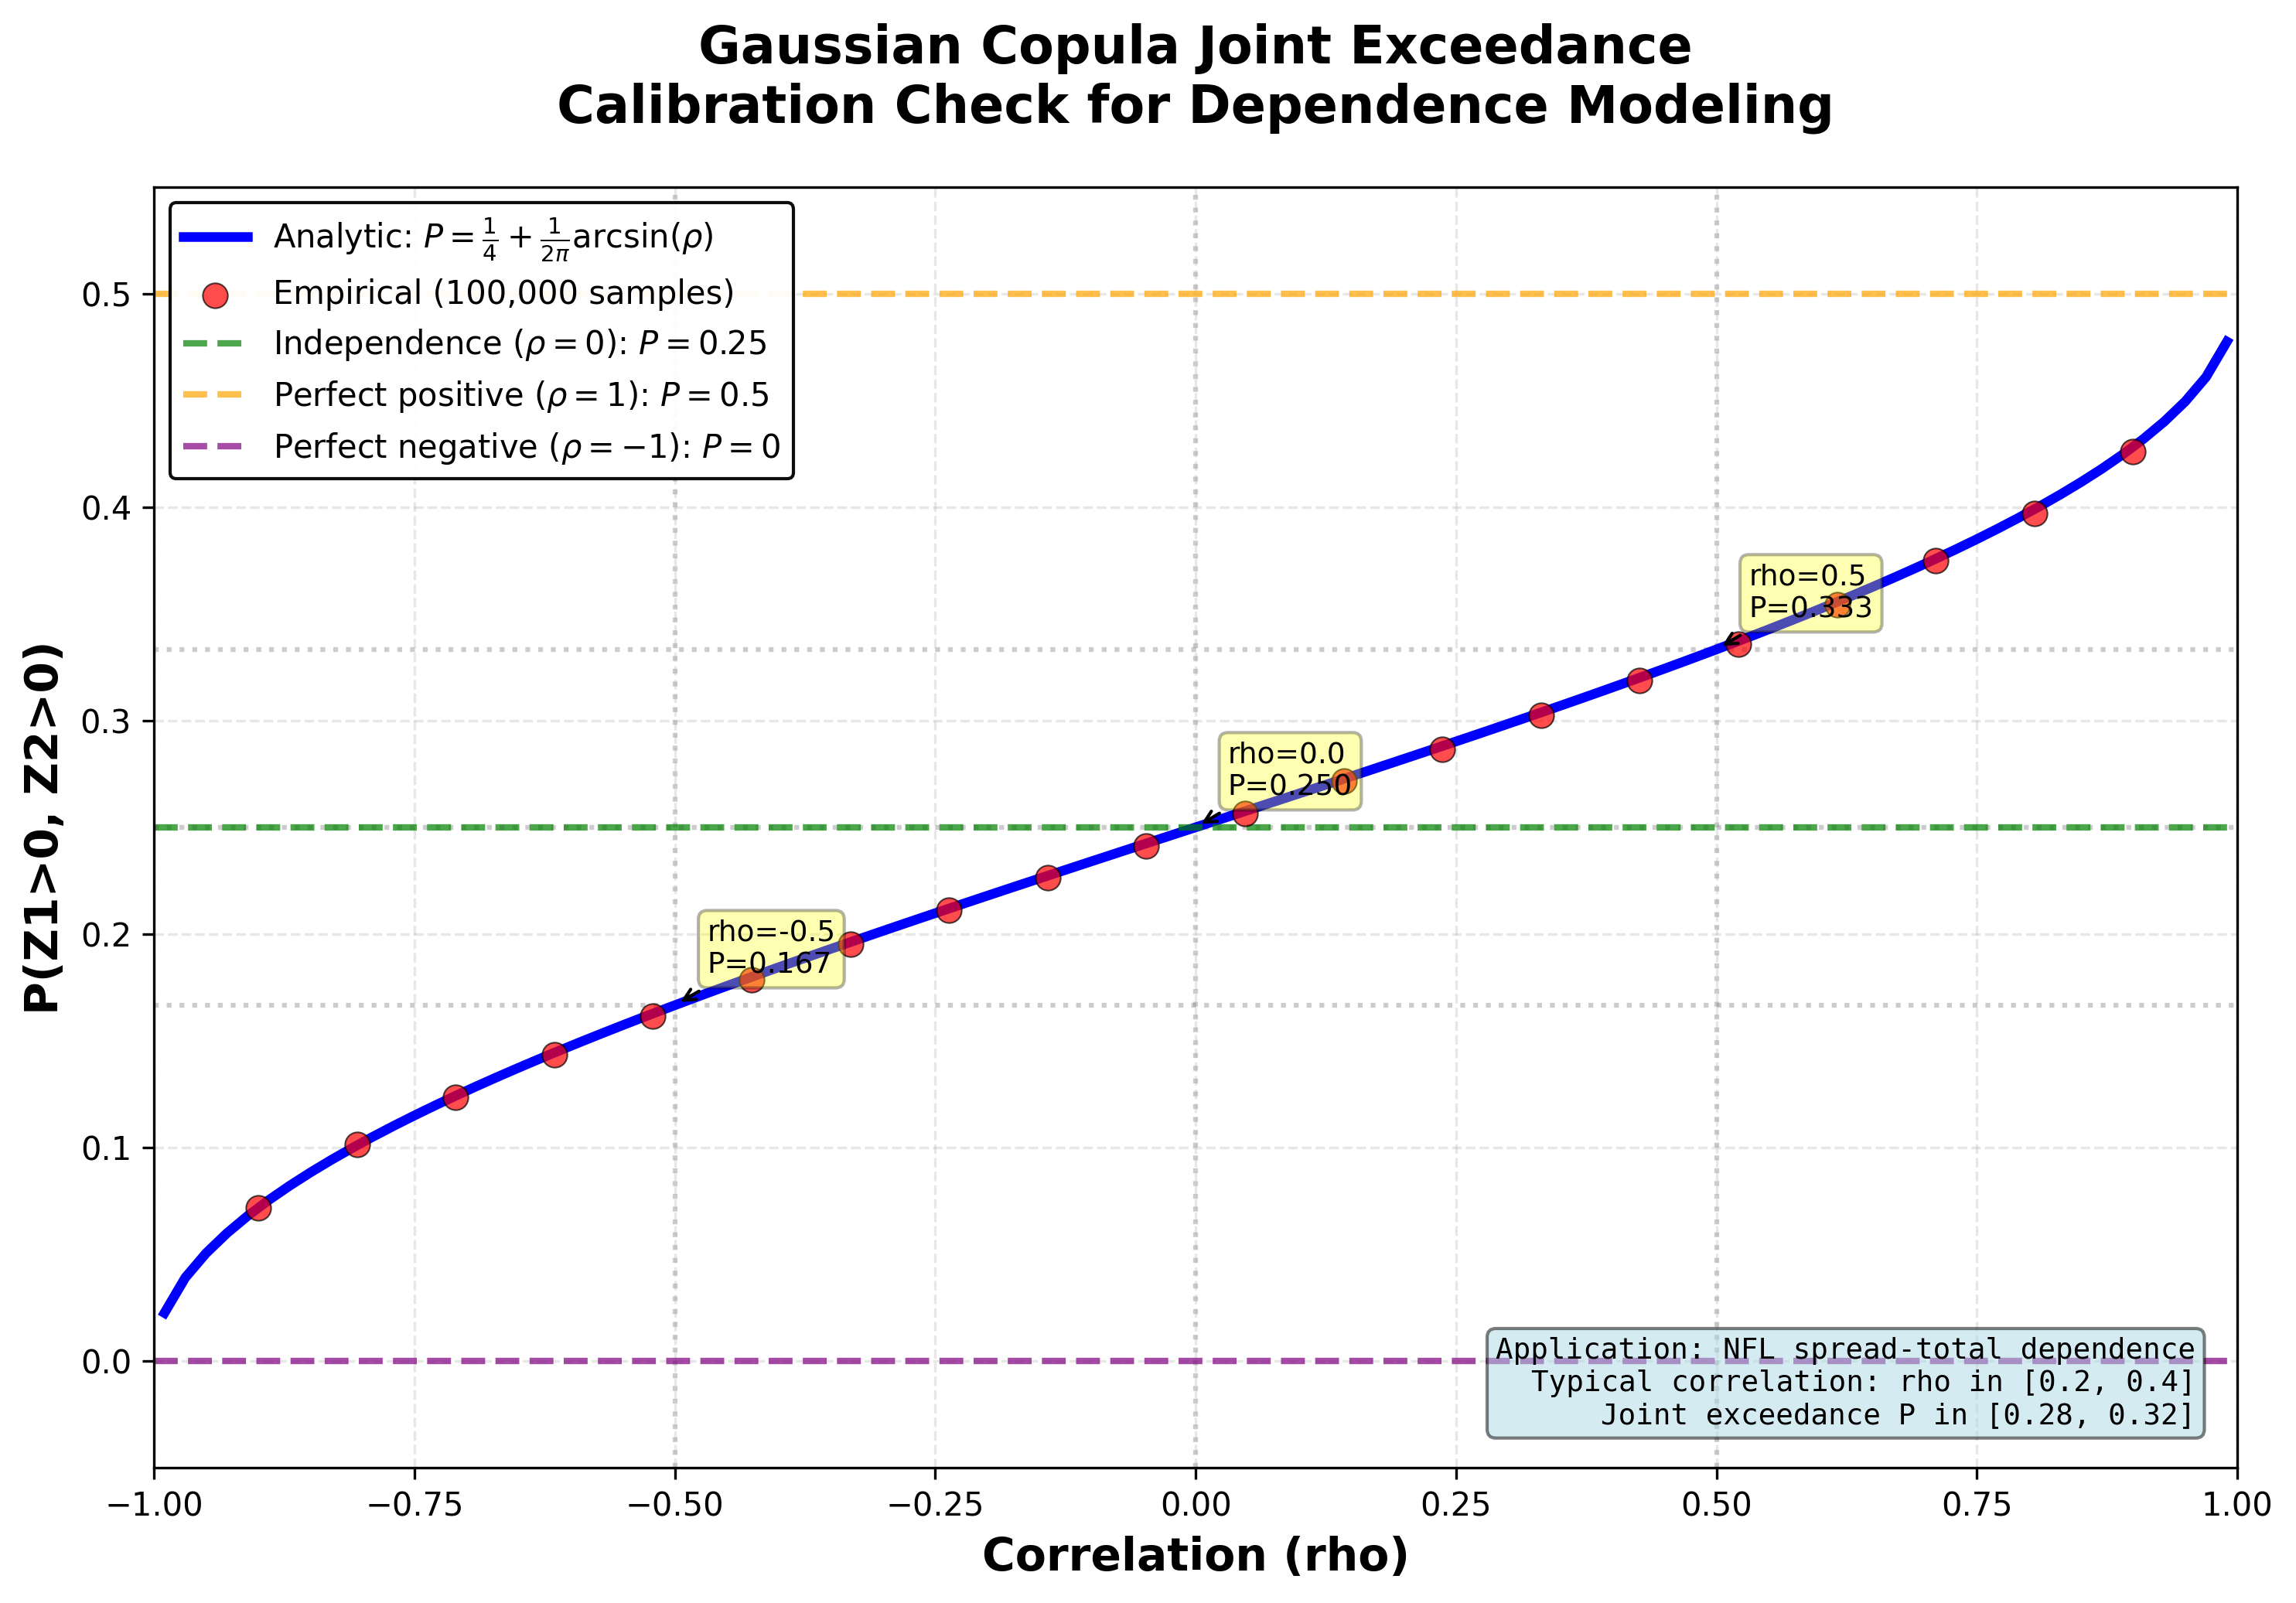
\includegraphics[width=0.9\linewidth]{../figures/joint_exceedance_vs_rho.png}
  \caption{Gaussian-copula joint exceedance at symmetric thresholds ($z_1=z_2=0$) as a function of correlation $\rho$. The analytic curve $\Prob(Z_1>0,Z_2>0)=\tfrac14+\tfrac{1}{2\pi}\arcsin(\rho)$ provides a calibration check for dependence modeling (\Cref{subsec:copula-st}).}
  \label{fig:copula-joint}
\end{figure}

\section{Tail Refinements and Approximations}
\subsection{Edgeworth and saddlepoint tail refinement}\label{subsec:edgeworth}
Let $M$ be integer margin with mean $\mu_D$, variance $\sigma_D^2$, standardized $Z=(M-\mu_D)/\sigma_D$,
skewness $\gamma_1$ and kurtosis $\gamma_2$. The Edgeworth approximation to $\Prob(M\le m)$ is
\[
\Phi(z)+\phi(z)\!\left(\frac{\gamma_1}{6}(z^2-1)+\frac{\gamma_2}{24}(z^3-3z)+\frac{\gamma_1^2}{72}(z^5-10z^3+15z)\right),
\]
$z=(m+\tfrac12-\mu_D)/\sigma_D$ (continuity-corrected). For lattice accuracy at extreme tails we also use
the saddlepoint approximation with cumulant generator $K(t)=\log \E[e^{tM}]$:
\[
\Prob(M=m)\approx \frac{1}{\sqrt{2\pi K''(\hat t)}}\exp\!\big(K(\hat t)-\hat t\,m\big),
\quad \text{with }K'(\hat t)=m.
\] \footnote{Classical accuracy results for saddlepoint/Edgeworth approximations include \citet{daniels1954}; see also \Cref{subsec:crps-lattice} for discrete-evaluation implications.}

\subsection{Restricted EM for Skellam under key constraints}\label{subsec:skellam-em}
Let $D_i$ be observed margins and $(\lambda,\mu)$ the Skellam parameters. Define a pseudo-complete
representation with latent $(X_i,Y_i)$ s.t.\ $D_i=X_i-Y_i$, $X_i\sim\mathrm{Pois}(\lambda)$,
$Y_i\sim\mathrm{Pois}(\mu)$. The E-step computes $\E[X_i\mid D_i]$ and $\E[Y_i\mid D_i]$
via Bessel identities; the M-step sets
\[
\lambda^{\text{new}}=\frac{1}{n}\sum_i \E[X_i\mid D_i],\qquad
\mu^{\text{new}}=\frac{1}{n}\sum_i \E[Y_i\mid D_i].
\]
To enforce key masses $\tilde q(k)=m_k$ ($k\in\mathcal{K}$), project $(\lambda,\mu)$ after the M-step
onto the feasible set $\{(\lambda,\mu): \sum_{d\in\mathbb{Z}} w_d(\lambda,\mu)q(d)=1,\ \tilde q(k)=m_k\}$.\footnote{See also \Cref{subsec:bp-pmf} and \citet{karlis2003} for related EM-style constructions in bivariate settings.}

% (Removed duplicative recaps of Bradley--Terry/Elo/Harville/Glickman--Stern; see Canonical Foundations \S\ref{subsec:harville1980}, \S\ref{subsec:glickman1998} and Paired-Comparison \S\ref{sec:paired} for the full treatment.)

\section{Score / Margin Distributions}
\label{sec:score}

\paragraph{Summary (pointers, not repeats).} To avoid duplication, we summarize the score/margin families used and point to the derivations already given:
\begin{itemize}
  \item \textbf{Independent Poisson with Dixon--Coles small-score reweighting:} see \Cref{subsec:maher1982,subsec:dixon1997}. We use this for quick calibration near low scores.
  \item \textbf{Bivariate Poisson (shared component):} see \Cref{subsec:karlis2003,subsec:bp-pmf}. This supplies coherent joint pricing for correlated legs.
  \item \textbf{Dynamic bivariate Poisson:} see \Cref{subsec:koopman2015} for the time-evolving formulation; we use it to let dependence shift through the season.
  \item \textbf{Skellam margins and key numbers:} construction/moments in \Cref{subsec:skellam1946,subsec:skellam-mom}; integer reweighting in \Cref{subsec:key-reweight,subsec:dc-vs-keys}.
  \item \textbf{Spread-to-win mapping:} derivation and usage in \Cref{subsec:stern1991,subsec:stern-derivation}.
  \item \textbf{Zero-inflated/hurdle variants:} used rarely for extreme low-scoring eras; orthogonal to integer-margin reweighting.
\end{itemize}

These components are the building blocks for simulation and pricing in Chapter~\ref{chap:sim}; we do not restate formulas here.

\section{Calibration, Scoring \& Uncertainty}
\label{sec:calib}

\subsection{Scoring Rules}
We evaluate models by:
\begin{itemize}
  \item \textbf{Brier score:} \( \frac{1}{N} \sum (p_i - y_i)^2 \)
  \item \textbf{Log-loss:} \( -\frac{1}{N} \sum [y_i \log p_i + (1-y_i)\log(1-p_i)] \)
  \item \textbf{Reliability diagrams, ECE:} partition probabilities into bins and check empirical frequency
\end{itemize}

% Reliability diagram with binomial confidence intervals
\begin{figure}[t]
  \centering
  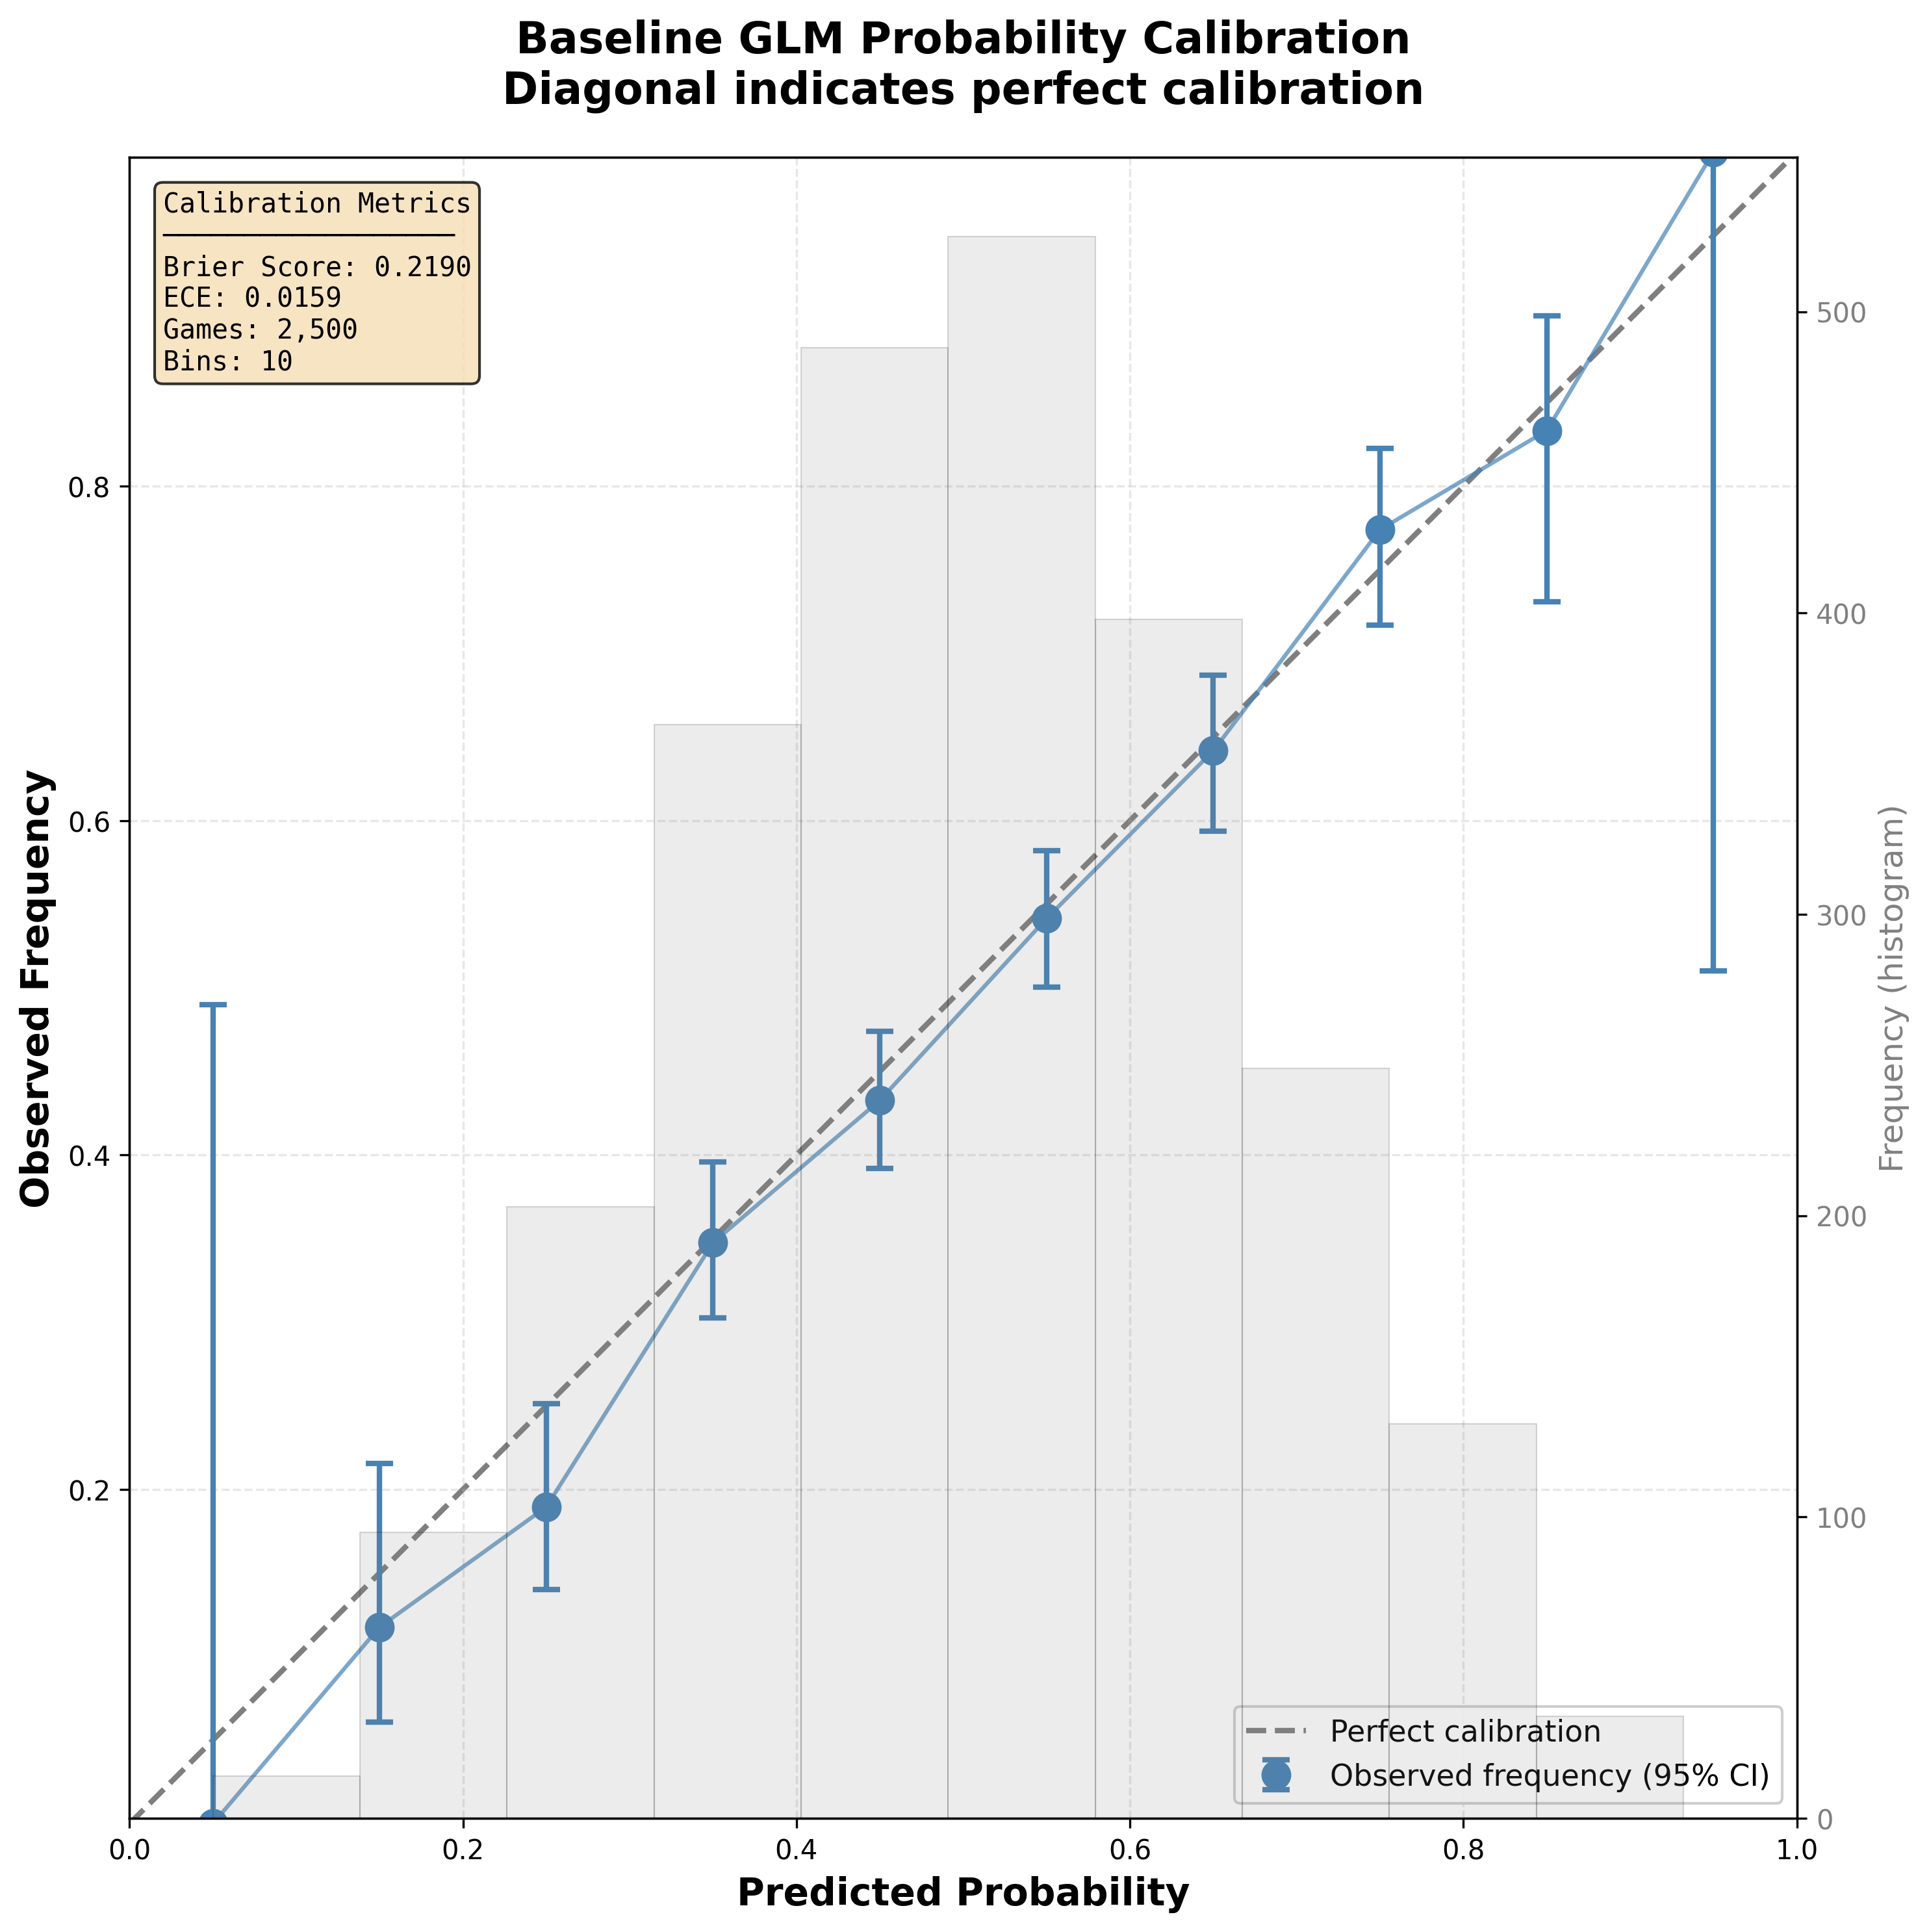
\includegraphics[width=0.9\linewidth]{../figures/reliability_diagram.png}
  \caption{Reliability diagram with 95\% binomial confidence intervals. Points show empirical frequencies by predicted-probability bin; the diagonal indicates perfect calibration. We report these alongside Brier/log-loss and ECE.}
  \label{fig:reliability}
\end{figure}

\subsection{Uncertainty Quantification}
Classical Bayesian/state-space models give posterior predictive distributions by default.  
For ML models, we will estimate predictive intervals via:
\begin{itemize}
  \item Bootstrapping over training subsets
  \item Quantile regression layers
  \item Ensemble variance
\end{itemize}
We propagate these intervals into staking decisions: bets with wide uncertainty may be filtered or heavily downweighted.

\subsection{Evaluation Protocols}
Temporal cross-validation, blocked by week and season, avoids leakage from future injuries and market moves. We report Brier score decomposition (reliability, resolution, uncertainty) and reliability diagrams with equal-frequency bins. For margin distributions we report CRPS and PIT histograms to check sharpness and calibration simultaneously.

\subsection{Robustness Checks}
We test sensitivity to era definitions (pre- and post-rule changes), outlier handling (wins above the 99th percentile), and class imbalance between favorites and underdogs. Where necessary, we employ robust losses and quantile calibration to maintain stability.

\section{Machine Learning Models in NFL Prediction}
\label{sec:ml}

\subsection{Vigorish removal and CBV}\label{subsec:vig-cbv-lit}
For two-outcome market with American odds $(o_1,o_2)$ convert to decimals $(d_1,d_2)$ and implied
probabilities $\pi_i^{\mathrm{raw}}=1/d_i$. The hold is $H=\pi_1^{\mathrm{raw}}+\pi_2^{\mathrm{raw}}-1$.
No-vig probabilities are $\pi_i=\pi_i^{\mathrm{raw}}/(1+H)$. Given model fair $\hat\pi_i$, the
comparative book value is
\[
\mathrm{CBV}_i=\hat\pi_i-\pi_i,
\]
or in price space $\Delta_i = d_i - (1/\hat\pi_i)$. We bet when $\mathrm{CBV}_i>\tau$ or $\Delta_i>\tau'$.

\subsection{Feature Sets and Interactions}
Key feature families include:
\begin{itemize}
  \item Efficiency metrics: EPA/play, success rate (offense, defense, by down/distance)
  \item Play-calling: PROE (pass rate over expected), pace (sec/play), pass vs run splits
  \item Trench indicators: pressure allowed/created, stuff rate, line yards proxies
  \item Roster \& injuries: QB status, adjusted games lost (AGL), starters out
  \item Environmental: weather (wind, rain, temp), turf/grass, altitude
  \item Market microstructure: implied probability, hold, line-move delta, cross-book spreads (CBV)
\end{itemize}

We use ML (e.g.\ gradient boosting, neural nets) to capture nonlinear interactions among these features, stacking with classical model outputs as base features.

\paragraph{Feature Interactions and Shifts.}
We devote special attention to interaction effects (e.g.\ weather by pass rate, injuries by team form) and to covariate shift between early and late season. Drift monitors track the distribution of CBV, EPA, and pace to trigger recalibration.

\subsection{Regularization, Calibration \& Robustness}
We guard against overfitting via:
\begin{itemize}
  \item Time-based cross-validation (rolling windows)
  \item Strong regularization (ridge, lasso, elastic net)
  \item Probability calibration (Platt scaling, isotonic regression) on held-out data
  \item Ensemble bootstraps and variance reduction
\end{itemize}

\section{Reinforcement Learning for Betting}
\label{sec:rl}

\subsection{MDP Formulation for Betting}
We treat each potential bet (pre-game or intra-game) as a step in an MDP:
\[
\begin{aligned}
s_t &= (\text{model predictions},\ \text{market state},\ \text{bankroll},\ \text{time}),\\
a_t &\in \{\text{no bet},\ \text{stake bucket}\},\\
r_t &= \text{PnL (or utility)}.
\end{aligned}
\]
Actions can include correlated bets across markets (spread + total) or hedges.

\subsection{RL Algorithms and Offline Training}
We experiment with:
\begin{itemize}
  \item \textbf{DQN / Q-learning}: discretized stake buckets, value iteration + experience replay
  \item \textbf{PPO / Actor–Critic}: continuous or stochastic stake policies, clipped updates, entropy regularization
  \item \textbf{Uncertainty-aware gating}: suppress stakes when posterior CI is wide (e.g.\ if variance too high)
\end{itemize}
We train offline (historical seasons) and optionally refine online via simulated paper-trading episodes.

\subsection{Off-Policy Evaluation}
Before deploying a learned policy, we estimate its value via inverse-propensity scoring, weighted importance sampling, and doubly robust estimators. We discuss variance control via self-normalization and clipping, and how model-based simulators can bias OPE if mis-specified.

\section{Game-Theoretic Foundations}
\label{sec:game-theory}
\subsection{Why game theory here?}
Bookmakers and bettors form a strategic ecosystem with asymmetric information, inventory constraints, and repeated interaction. Pre‑game pricing is well approximated by a Stackelberg game: the bookmaker (leader) posts odds and limits anticipating heterogeneous follower responses; many small bettors act approximately as price‑takers.

\subsection{Mathematical framing}
Two simple primitives illuminate the trade‑offs:
\begin{itemize}
  \item \textbf{Risk‑aware market maker.} Let $\pi$ be prices (implied probs) and $Q(\pi)$ the net demand vector. With outcome randomness $\theta$, one stylized objective is
  \[
  \max_{\pi}\; \E_\theta[\Pi(\pi;\theta)]\,-\,\lambda\,\Var_\theta[\Pi(\pi;\theta)]\,-\,\gamma\,\|Q(\pi)\|_2^2,
  \]
  where $\lambda,\gamma\ge 0$ encode risk and inventory costs. First‑order conditions imply \emph{price shading} against imbalanced flow, increasing with outcome variance and demand inelasticity (bias), helping explain vig width and line tilts.
  \item \textbf{Kelly bettor as log‑utility agent.} For decimal odds $d$ and success probability $p$, the stake fraction $f$ that maximizes $\E[\log(1+fR)]$ with $R\in\{d-1,-1\}$ is $f^\star=\tfrac{dp-1}{d-1}$ when $dp>1$, else $0$. Under uncertainty, replacing $p$ by a lower confidence bound yields the Kelly‑LCB rule used as a baseline and connects to CVaR sizing (Chapter~\ref{chap:risk}).
\end{itemize}

\subsection{NFL market applications}
\begin{itemize}
  \item \textbf{Adverse selection and limits.} Lines move with injuries/weather because informed flow arrives; books mitigate loss via limits and shading. Our features include line velocity and cross‑book deltas to proxy information arrival.
  \item \textbf{Equilibrium and efficiency.} Closing prices approximate a competitive equilibrium; persistent positive CLV/ROI indicates deviations conditional on frictions. Our evaluation explicitly tests this.
  \item \textbf{Dynamic interaction.} Live betting is a dynamic game with inventory feedback; pre‑game in this work assumes small, price‑taking stakes so odds are exogenous to the policy (offline RL setting).
  \item \textbf{Correlation risk.} Books manage portfolio risk across legs; our copula layer and CVaR constraints mirror this at bettor scale for teasers/SGPs.
\end{itemize}

\subsection{Testable implications}
Game‑theoretic frictions predict pockets of inefficiency where (i) inventory/rounding bites (key numbers), (ii) information latency is high (late injury/weather), or (iii) demand is biased (favorites/popular teams). Our ablations target exactly these loci: key‑number reweighting, microstructure features, and copula choice.

\section{Betting Market Theory \& Microstructure}
\label{sec:market}

\subsection{Economics of Wagering Markets}
Sauer (1998) surveys the structure and efficiency of wagering markets, including bookmaker margins, bettor behavior models, and informational asymmetries. \citep{sauer1998}  
Levitt (2004) argues bookmakers sometimes exploit bettor biases (e.g. overbetting favorites) rather than purely balancing books. \citep{levitt2004}

\subsection{Closing-Line Efficiency and Biases}
We review evidence that the closing line aggregates information efficiently on average, yet exhibits pockets of bias around key numbers and popular teams. Behavioral patterns (favorite-longshot bias, recency effects) appear in subsets of the market and motivate features that measure retail pressure and line velocity.

\subsection{Cross-Market Dependence}
Spreads, totals, and moneylines are not independent. We discuss correlation structures induced by shared latent team strength and tempo, and implications for correlated parlays and hedging.

\subsection{Market as Signal and Benchmark}
We treat the market (closing lines) as both:
\begin{itemize}
  \item A performance benchmark: our models must outperform or capture CLV (closing line value) edge
  \item A feature: cross-book spreads, line velocity, implied vs model delta, push rules
\end{itemize}
We define **Comparative Book Value (CBV)** as the difference between our fair probability and implied market probability; large CBV signals potential mispricing worth a bet.

\section{Design Synthesis and Implications}
\label{sec:synth}

\begin{table}[p]
  % Center this float vertically on its own page
  \vspace*{\fill}
  \centering
  % Slightly extend into the side margins for this table only
  \begin{adjustwidth}{-0.35in}{-0.35in}
  \begin{threeparttable}
  \captionsetup{justification=centering}
  \caption{Modeling families at a glance. Uncertainty, scalability, interpretability, and notes for deployment.}
  \label{tab:model-compare}
  \begingroup
   \small
   \setlength{\tabcolsep}{6pt}%
   \renewcommand{\arraystretch}{1.25}% more space between rows
   \setlength{\aboverulesep}{0.6ex}% spacing around rules
   \setlength{\belowrulesep}{0.5ex}%
   \begin{tabularx}{\linewidth}{@{} l Y Y Y Y @{} }
     \toprule[1.2pt]
     \textbf{Model} & \textbf{Uncertainty} & \textbf{Scalability} & \textbf{Interpretability} & \textbf{Deployment notes} \\
     \midrule
     Harville LMM & analytic posteriors & high & high & rapid weekly updates; Gaussian residuals assumption \\
     Glickman--Stern & full posterior (Kalman/MCMC) & moderate & medium & priors clarify drift; MCMC cost at scale \\
     Dixon--Coles & low-score reweight & high & high & quick key-number recalibration \\
     Bivariate Poisson & parametric/joint draws & moderate & medium & handles correlation; initialization sensitive \\
     ML ensembles & ensemble variance & high & low & monitor drift via attributions \\
     RL policy & bootstrap + MC & moderate & medium & risk gating via CVaR; compute intensive \\
     \bottomrule[1.2pt]
   \end{tabularx}
  \endgroup
  \begin{tablenotes}[flushleft]\footnotesize
    \item Notes: qualitative ratings; see \Cref{subsec:harville1980,subsec:glickman1998,subsec:maher1982,subsec:dixon1997,subsec:karlis2003,subsec:koopman2015} for derivations and Chapter~\ref{chap:rl} for policy design.
  \end{tablenotes}
  \end{threeparttable}
  \end{adjustwidth}
  % Vertical centering end
  \vspace*{\fill}
\end{table}

From the literature, our design principles are:
\begin{enumerate}
  \item Use Bayesian / shrinkage models to generate priors and uncertainty bounds.
  \item Use discrete margin / score distributions (bivariate Poisson + reweight) to price spreads, totals, teasers.
  \item Use ML meta-models to absorb nonlinear interactions among features.
  \item Use RL to convert edges into action sequences under risk constraints.
  \item Leverage the market as both a signal and benchmark; bet only when CBV passes threshold.
\end{enumerate}

\bigskip
% Integer-margin PMF comparison: baseline vs key-number reweighted
\begin{figure}[t]
  \centering
  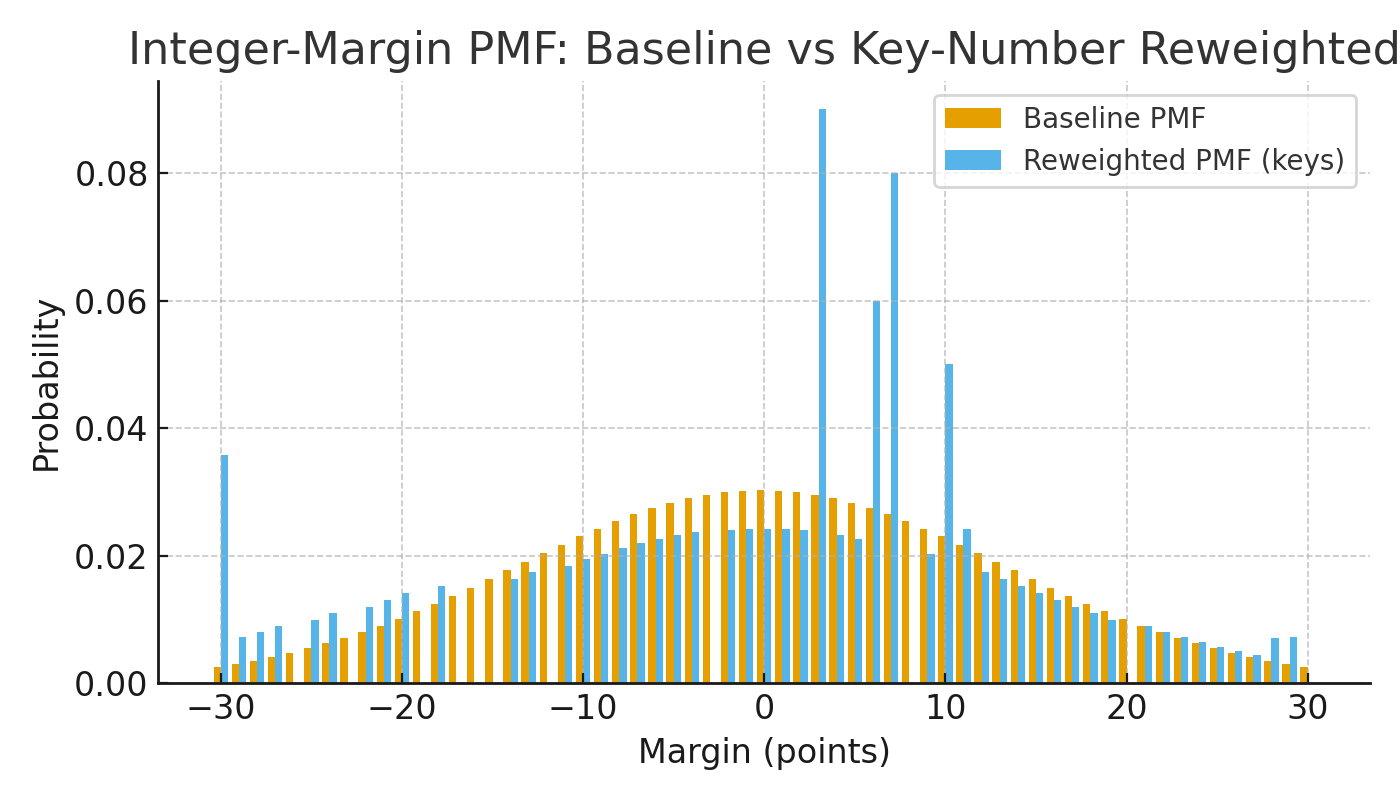
\includegraphics[width=\linewidth]{../figures/key_number_pmf.png}
  \caption{Integer-margin pmf comparison. Baseline (e.g., Skellam/discretized Gaussian) vs key-number reweighted distribution matching empirical masses at 3, 6, 7, and 10 while preserving location/scale (\Cref{subsec:key-reweight}).}
  \label{fig:key-pmf}
\end{figure}

\section{Annotated Reading List}
We provide brief annotations of representative works that inform the hybrid design:
\begin{itemize}
  \item \citet{harville1980}: Linear mixed models for NFL margins; interpretable and fast with shrinkage via BLUP. Serves as a reliable baseline and prior.
  \item \citet{glickman1998}: State-space dynamics for team strength with Bayesian inference; enables credible intervals and smooth drift handling.
  \item \citet{stern1991}: Mapping spread to win probability via normal approximation; practical bridge between margin and moneyline pricing.
  \item \citet{dixon1997}: Independent Poisson with low-score adjustment; cornerstone for discrete score modeling in low-scoring sports.
  \item \citet{karlis2003}: Bivariate Poisson with shared component to capture correlation; essential for teaser/parlay risk modeling.
  \item \citet{koopman2015}: Dynamic Poisson intensities with simulation-based filtering; template for time-varying scoring rates.
  \item \citet{lock2014}: Random-forest win probability at play-level; illustrates ML gains and calibration considerations for football.
  \item \citet{sauer1998}: Economics of wagering markets; frames bookmaker margins, bettor behavior, and informational asymmetry.
  \item \citet{levitt2004}: Bookmaker objectives and bettor biases; motivates microstructure features and bias-aware evaluation.
  \item \citet{szalkowski2012}: Collective wisdom of lines; closing prices as an efficient benchmark with pockets of inefficiency.
  \item \citet{nichols2014}: Time-zone effects on performance; supports travel/rest features in predictive models.
  \item \citet{baio2010}: Bayesian hierarchical football models; demonstrates full-probabilistic inference benefits for uncertainty quantification.
\end{itemize}

\section{Canonical Works Integrated}
\label{sec:canon}
We explicitly compare and implement: Harville (1980), Glickman–Stern (1998), Stern spread mapping (1991), Dixon–Coles (1997), Karlis–Ntzoufras (2003), Koopman dynamic Poisson (2015), Lock \& Nettleton (2014), Sauer (1998), Levitt (2004).  
Implementation, ablation, and critique will occur in Chapter~\ref{chap:methods}.

\section{Classical vs Modern: A Comparative Synthesis}
Classical models provide structure, interpretability, and tractable uncertainty, while modern ML models absorb nonlinear interactions and idiosyncrasies that generative assumptions miss. The hybrid approach leverages classical models for priors and calibration discipline, layering ML for residual structure and using RL to translate edges into actions under explicit constraints. This division of labor prevents ML from overfitting low‑signal regimes and keeps decision‑making grounded in uncertainty.

\subsection{When Classical Wins}
In data‑scarce or rapidly shifting regimes (e.g., early season, injury turbulence), shrinkage and state‑space models dominate due to better calibrated uncertainty and temporal smoothing. Their transparent parameters support operational overrides.

\subsection{When ML Wins}
With stable covariates and rich features (market microstructure, team‑form interactions), ML ensembles produce sharper probabilities. Calibration layers (Platt, isotonic) restore reliability while preserving sharpness.

\subsection{Bridging to Decision Value}
Sharpness without calibration harms staking; calibration without sharpness limits EV. We therefore co‑optimize for proper scoring rules and enforce economic gates (CBV thresholds, variance caps) to realize value.

\section{From Score Distributions to Strategy}
Discrete score distributions support actionable constructs: teaser planning around key numbers, middle opportunities when line drift occurs, and hedges conditioned on joint outcomes. Reweighting Skellam/Poisson mass at integers aligns simulated legs with observed push probabilities, preventing systematic teaser mispricing. The bivariate Poisson’s shared component parameter governs correlation risk across legs; governance caps adjust as this parameter rises.

\section{Calibration Theory and Scoring Rules}
We review proper scoring rules for probability forecasts (log‑loss, Brier) and for full distributions (CRPS), highlighting the trade‑off between calibration and sharpness. We discuss reliability diagrams with binning bias corrections and isotonic/probit calibration approaches.

\section{Mapping Models to Decision Value}
We connect statistical metrics to economic outcomes by writing expected value (EV) and closing‑line value (CLV) explicitly in terms of probabilities and then linearizing the impact of probability error.

Consider a binary wager with decimal odds $d$ and true success probability $p$. The EV per unit stake is
\[\mathrm{EV}(p;d)=p\,d-1.\]
If the book is no‑vig with implied $\pi=1/d$, then $\mathrm{EV}(p;\pi)=p/\pi-1$. With a model probability $\hat p=p+\varepsilon$, the EV we act on is
\[\mathrm{EV}(\hat p;\pi)=\frac{\hat p}{\pi}-1=\frac{p}{\pi}-1+\frac{\varepsilon}{\pi}.\]
Hence, conditional on placing the bet, the first‑order EV error is $\varepsilon/\pi$. Averaging over bets, the mean absolute EV shortfall is controlled by the RMSE of $\varepsilon$; in particular, the Brier score $\E[\varepsilon^2]$ upper‑bounds the average EV loss up to the scale factor $1/\pi^2$.

Selection adds a gating effect: trades are taken only when $\hat p\ge \pi+\tau_\pi$ (a no‑vig threshold plus a margin for friction $\tau_\pi$). Near the threshold, a Taylor expansion shows false positives/negatives occur with probability proportional to the density of $\hat p$ at $\pi$, and their EV impact scales with the slope $\partial\,\mathrm{EV}/\partial p\big|_{p=\pi}=1/\pi$. Thus reducing calibration error (Brier/RMSE) and sharpening uncertainty (smaller variance of $\hat p$ near $\pi$) jointly improves realized EV.

In price space, let comparative book value $\mathrm{CBV}=\hat p-\pi$. Ignoring friction, $\mathrm{EV}\approx \mathrm{CBV}/\pi$; with slippage/fees $\tau$ and fill limits $c$, the executable EV is $\max\{0,\ \mathrm{CBV}/\pi-\tau\}$ with stake capped by $c$. This is why we optimize strictly proper scores (log‑loss, Brier/CRPS) while monitoring EV/CLV degradation from slippage and limits.

\section{Market Efficiency and Bias Tests}
We outline simple tests for favorite‑longshot bias, key‑number mispricing, and cross‑book arbitrage signals, emphasizing multiple‑testing corrections and robust standard errors.

\section{Synthesis and Open Questions}
The surveyed literature illustrates a continuum from interpretable generative models to flexible discriminative and sequential decision methods. Open challenges include (i) reconciling calibration with sharpness under distribution shift, (ii) integrating market microstructure without double-counting information, and (iii) handling multi-objective trade-offs between growth and risk in an operational setting. We outline how the hybrid approach in later chapters addresses these in a modular way that eases future extensions.

\section{Related Work Beyond Football}
Insights from other sports transfer imperfectly but inform modeling choices, particularly for low-scoring games (soccer, hockey) where Poisson-type models excel and for sequential decision domains (basketball substitutions, baseball bullpen management) where RL ideas have matured. We adapt ideas on tempo, possession value, and injury priors to the NFL context.

\section{Extended Notes on Calibration}
Calibration is both a statistical and an operational concern. A predictor can be perfectly calibrated and yet economically uninteresting if it lacks resolution; conversely, extremely sharp predictions can be economically harmful if they are miscalibrated. We therefore emphasize a portfolio of diagnostics: reliability diagrams with uncertainty bands, calibration slope/intercept for binary outcomes, PIT histograms for distributions, and CRPS to integrate sharpness and calibration into a single score. We also highlight the practical benefits of over-conservative probability outputs in risk-constrained decision problems.

\section{Liquidity, Limits, and Execution}
Modeling performance cannot be divorced from execution. Liquidity varies by book, time to kickoff, and market type. We discuss how to translate an estimated edge into an executable stake given posted limits and depth, and the implications for policy evaluation when some recommended bets cannot be filled at quoted prices. Execution-aware evaluation reduces optimism from paper backtests and promotes policies that scale gracefully.

\section{Teasers and Parlays}
Teasers (point adjustments for changed odds) and parlays (multiple legs) are common strategy components. We interpret them through joint distributions and correlation risk. A teaser can be attractive when key-number probabilities are underpriced; correlated parlays can be rational when the joint distribution assigns high mass to specific co-movements (e.g., low totals and underdogs). We caution that naive independence assumptions can be severely misleading.

For the full EV geometry and simulator context, see the teaser surface in Chapter~\ref{chap:sim} (\Cref{fig:sim-teaser-surface}).
\subsection{CRPS on lattices: propriety sketch}\label{subsec:crps-lattice}
For integer margins we work with a lattice distribution $F$ on $\mathbb Z$. The CRPS can be written as
\begin{equation}
\mathrm{CRPS}(F,y)=\sum_{m\in\mathbb Z} \big(F(m)-\mathbb 1\{m\ge y\}\big)^2\,\Delta_m,\qquad \Delta_m=1,
\end{equation}
which is the discrete analogue of the $L^2$ distance between $F$ and the step function at $y$. Taking expectation w.r.t. the true $Y\sim F^\star$ yields
\[\mathbb E\,\mathrm{CRPS}(F,Y)= \|F-F^\star\|_{L^2}^2 + \text{const},\]
since $\mathbb E\,\mathbb 1\{m\ge Y\}=1-F^\star(m-1)$. Hence the unique minimizer is $F=F^\star$, showing strict propriety on the lattice. This argument mirrors the continuous case in \Cref{subsec:gneiting2007}.

\chaptersummary{
This chapter connected classical models (Harville, Stern, Poisson/Skellam, bivariate/dynamic Poisson) to the practical needs of NFL betting: calibrated probabilities, realistic integer margins, and coherent dependence for multi‑leg bets. We established evaluation tools (CRPS, reliability) and introduced key‑number reweighting and copula‑based dependence as recurring motifs. Together these elements form the modeling pillar of the thesis that a hybrid stack with explicit uncertainty and governance transforms edge into reliable bankroll growth.
}{
Next we operationalize the data layer that feeds these models: reproducible ingestion, TimescaleDB marts, and feature catalogs (situational, team form, market, roster) in Chapter~\ref{chap:data}.
}
